\documentclass[10pt]{beamer}
\usepackage[utf8]{inputenc}
\usepackage{hyperref}
\hypersetup{colorlinks=true,linkbordercolor=blue,linkcolor=white,urlcolor=blue,pdfborderstyle={/S/U/W 1}}

\usepackage[scaled]{helvet}
\usepackage[T1]{fontenc}
\usetheme{Berkeley}
\beamertemplatenavigationsymbolsempty
\setbeamertemplate{headline}{}
\setbeamersize{sidebar width left=1.5cm}
\setbeamerfont{section in sidebar}{size=\fontsize{6}{6}\selectfont}
\setbeamerfont{title in sidebar}{size=\fontsize{6}{6}\selectfont}
\title{Geo-Visualization}
\date{}

\begin{document}
\maketitle

\section{Topics}
\begin{frame}
\leftskip1em\textbf{Learn}
	\begin{itemize}
    \item to visualize the delivery network on a map.
		\item about the advantages of selecting stations in the graph mode and in the GIS mode.
	\end{itemize}
\end{frame}

\section{1}
\begin{frame}
	\begin{center}
  		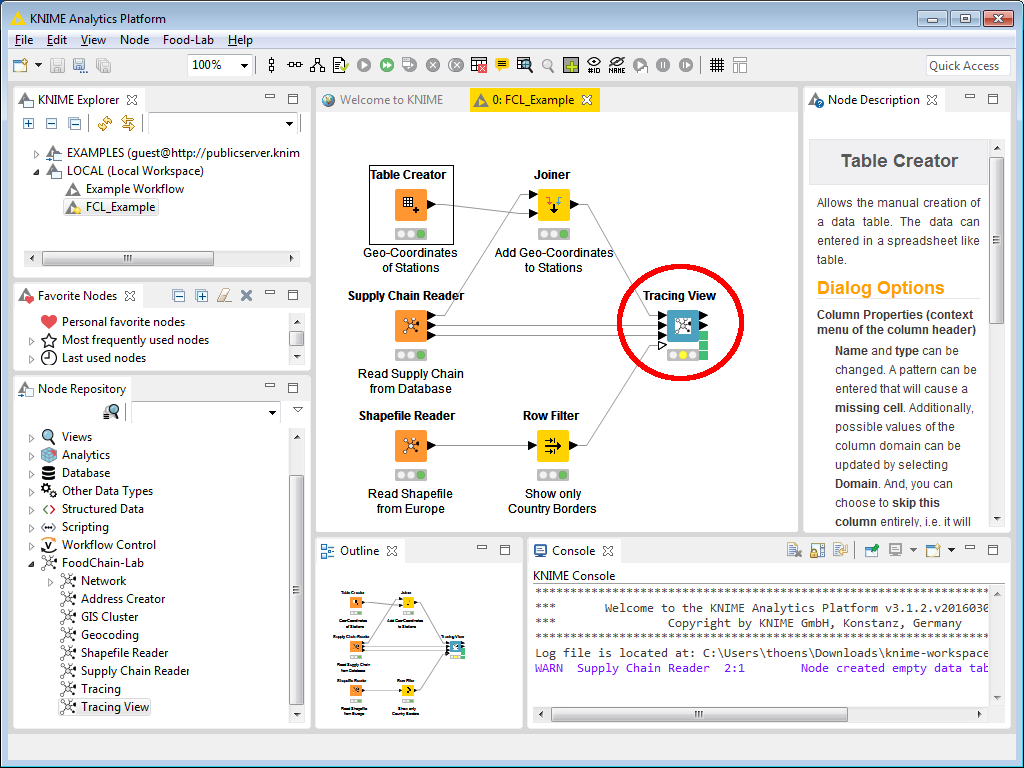
\includegraphics[height=0.6\textheight]{1.png}
	\end{center}
	\begin{itemize}
		\item Import the Example Workflow from \textcolor{blue}{\underline{\href{https://github.com/SiLeBAT/BfROpenLabResources/raw/master/GitHubPages/workflows/FCL\_Example.zip}{``FCL\_Example.zip''}}}.
		\item Open the \textbf{Tracing View} by double-clicking on it.
	\end{itemize}
\end{frame}

\section{2}
\begin{frame}
	\begin{center}
  		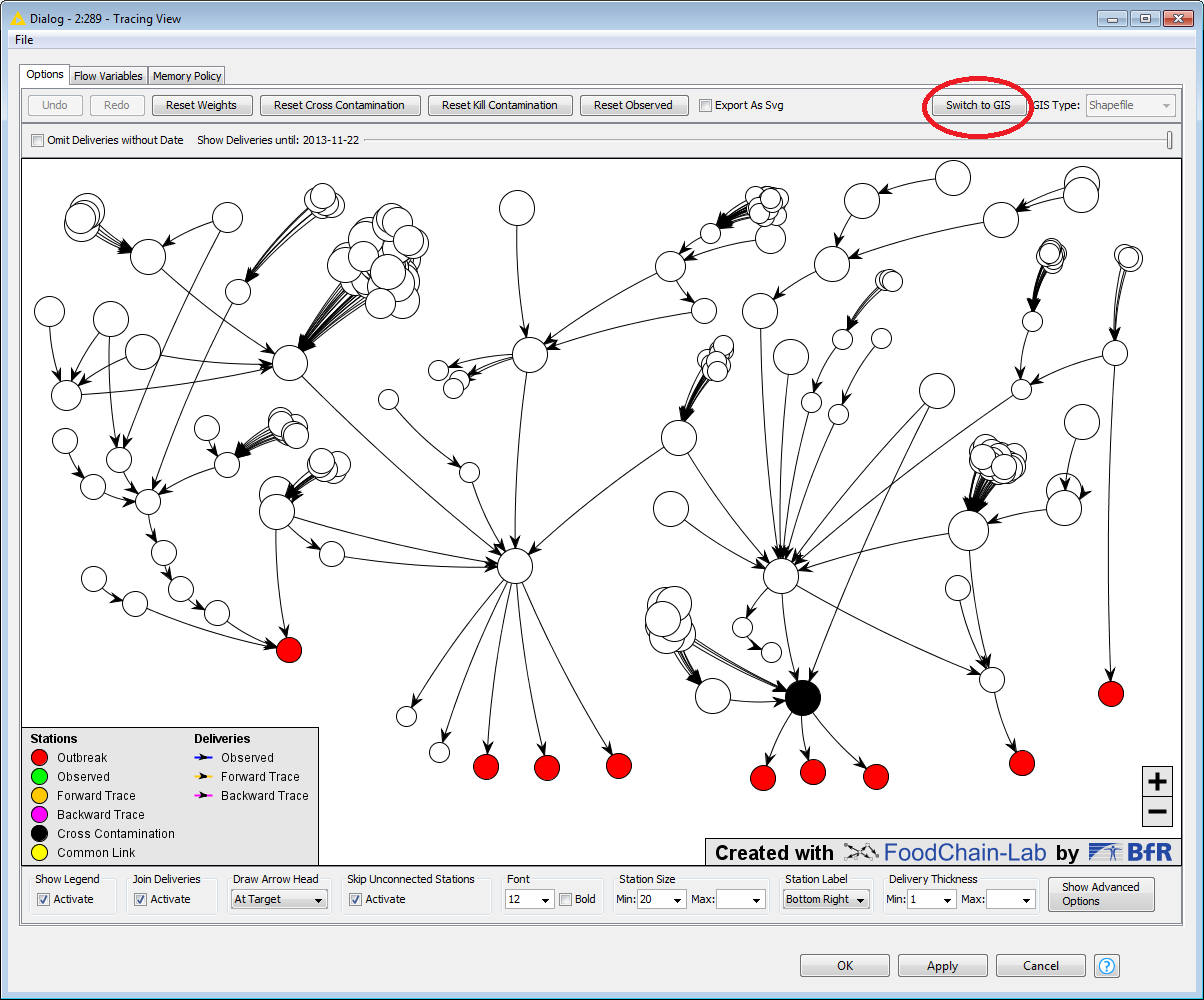
\includegraphics[height=0.6\textheight]{2.png}
	\end{center}
	\begin{itemize}
		\item Now you should see a graphical representation of the delivery network.
		\item To switch to the geographical representation click ``Switch to GIS'' in the upper right corner.
	\end{itemize}
\end{frame}

\section{3}
\begin{frame}
	\begin{center}
  		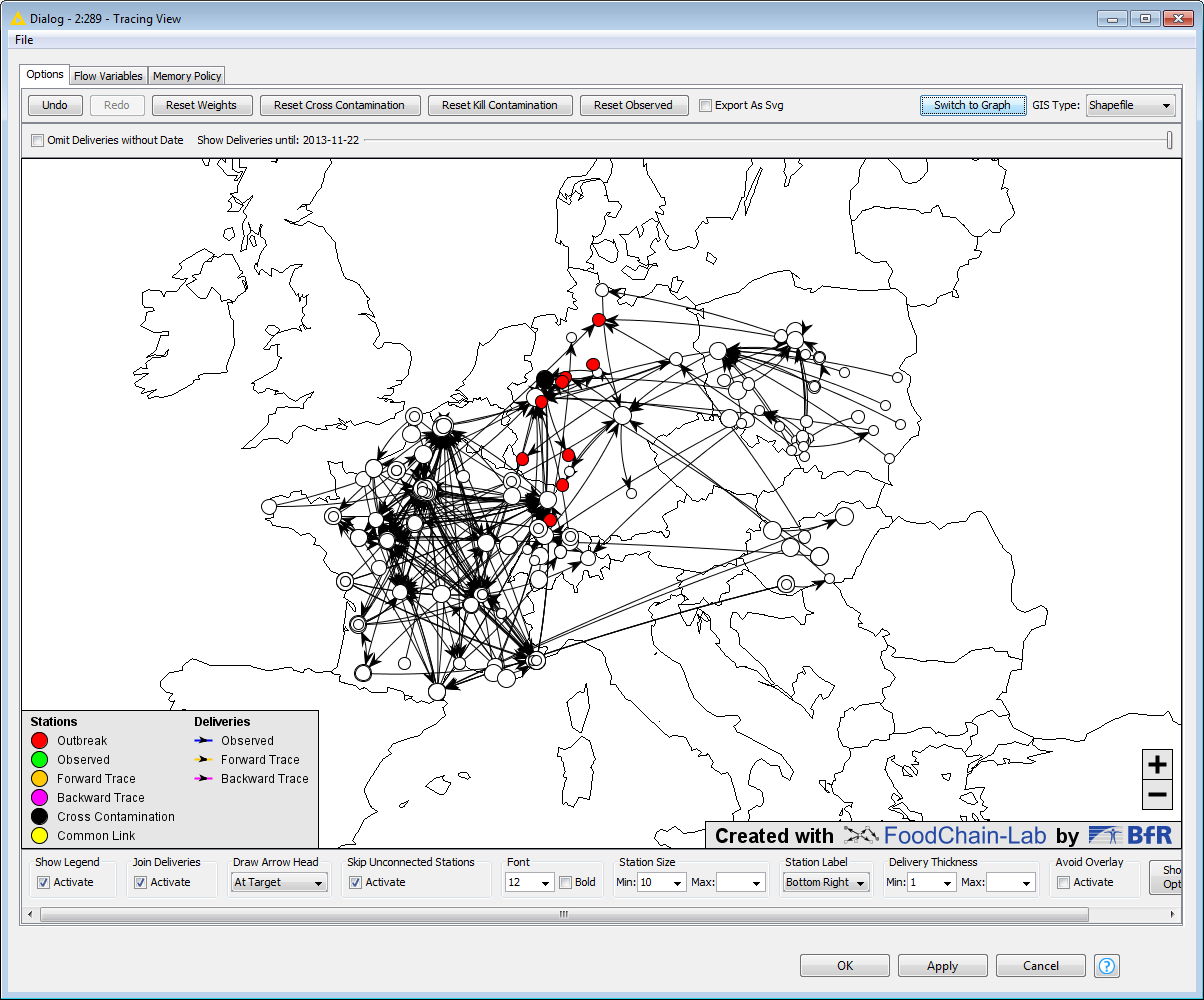
\includegraphics[height=0.6\textheight]{3.png}
	\end{center}
	\begin{itemize}
		\item The country borders originate from a shapefile which has been included in the KNIME workflow via the \textbf{Shapefile Reader}. Shapefiles are a good way to visualize networks on a map if there is no internet connection.
		\item To zoom to a certain area of the graph use the mouse wheel. By pressing down the left mouse button and moving the mouse you can move the map (works as in Google Maps).
	\end{itemize}
\end{frame}

\section{4}
\begin{frame}
	\begin{center}
  		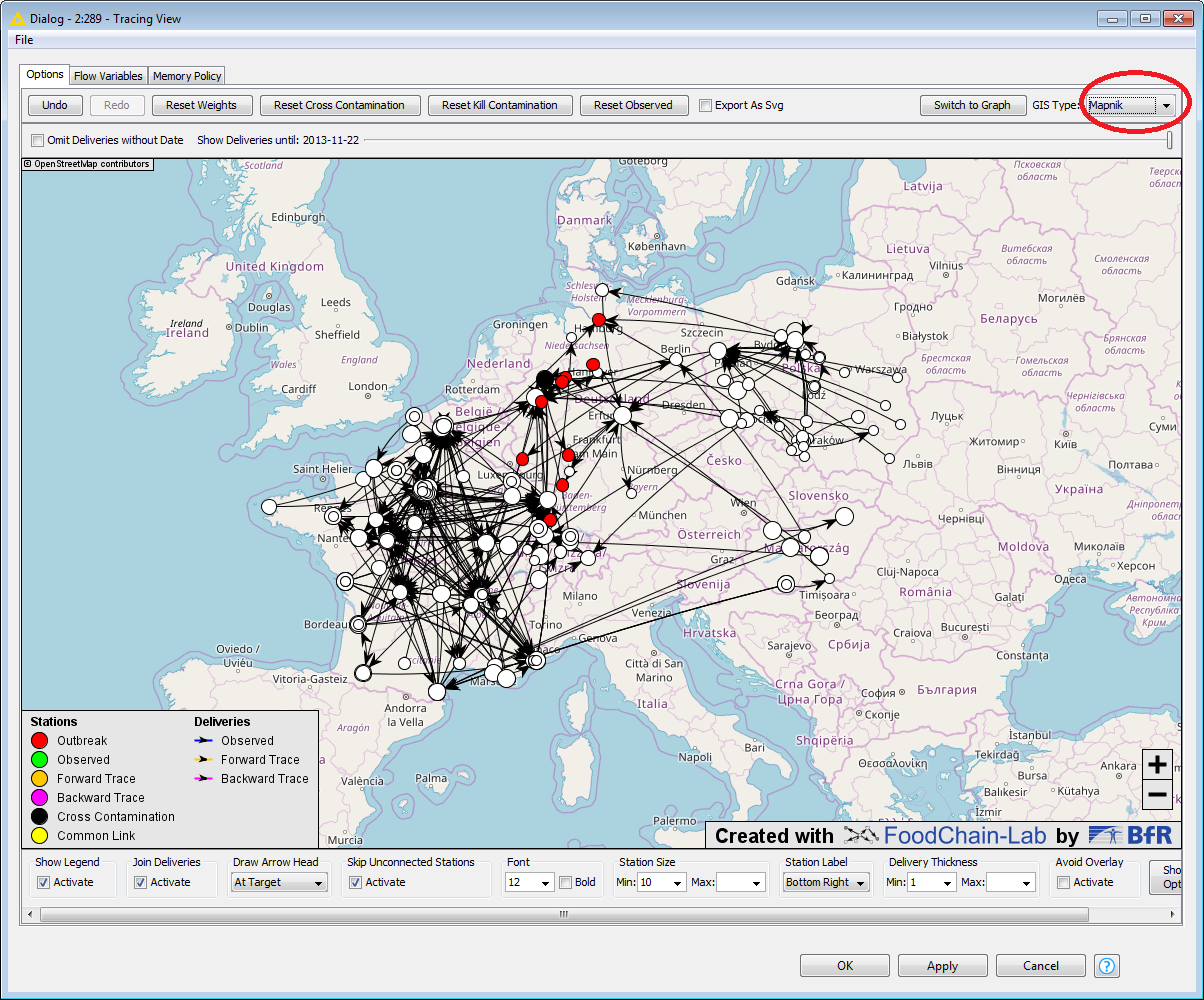
\includegraphics[height=0.6\textheight]{4.png}
	\end{center}
	\begin{itemize}
		\item If you are online, you can change the GIS Type. If you select ``Mapnik'', for example, you can see a visualization with OpenStreetMap data.
	\end{itemize}
\end{frame}

\section{5}
\begin{frame}
	\begin{center}
  		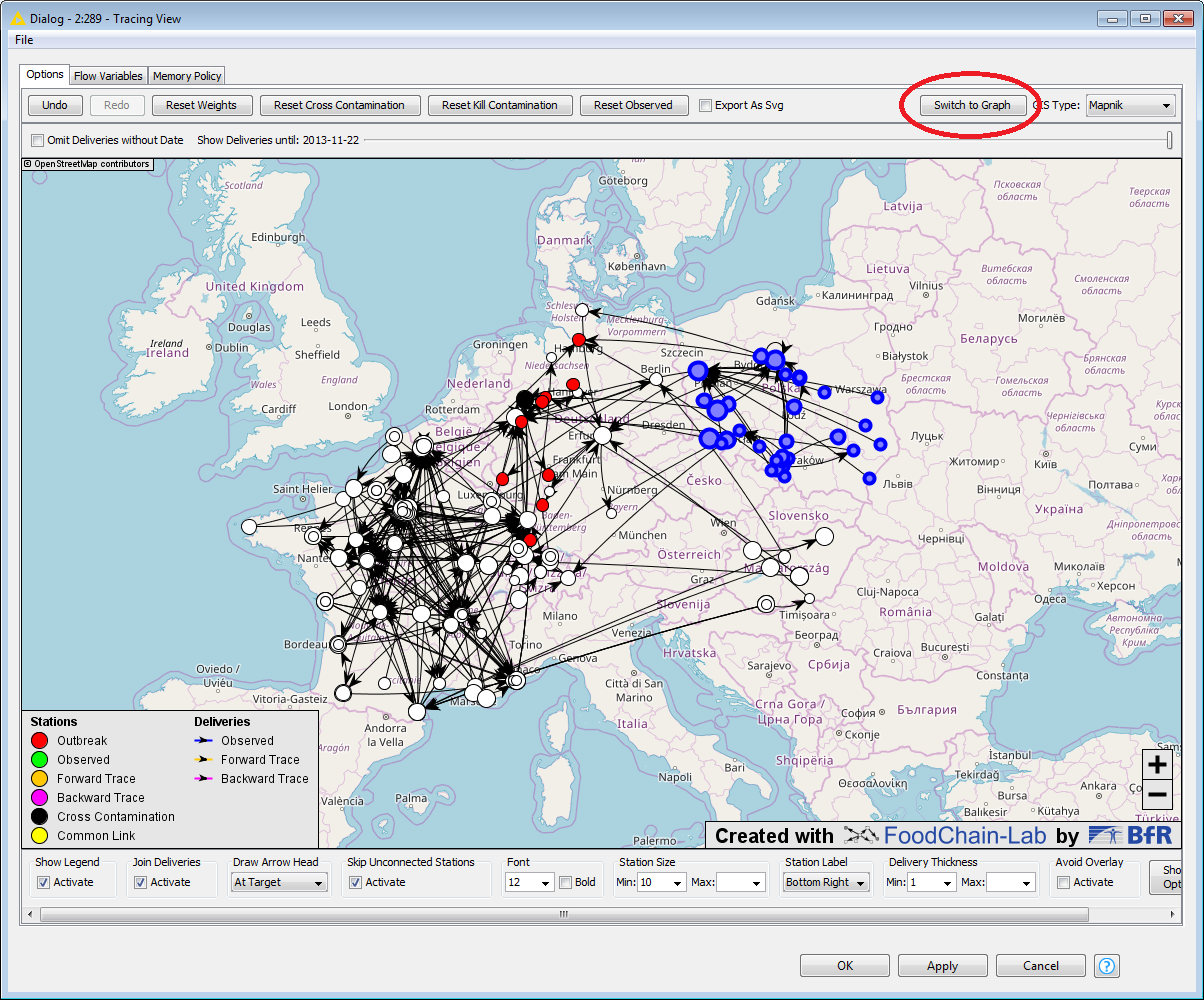
\includegraphics[height=0.55\textheight]{5.png}
	\end{center}
	\begin{itemize}
		\item We can now select certain stations based on geography: To select all stations in Poland press the ``Shift'' key on the keyboard, press the left mouse button and drag with the mouse a rectangle around the stations (everything at the same time).
		\item The selected stations are now colored blue.
		\item Switch back to the graphical view by clicking ``Switch to Graph'' in the upper right corner.
	\end{itemize}
\end{frame}

\section{6}
\begin{frame}
	\begin{center}
  		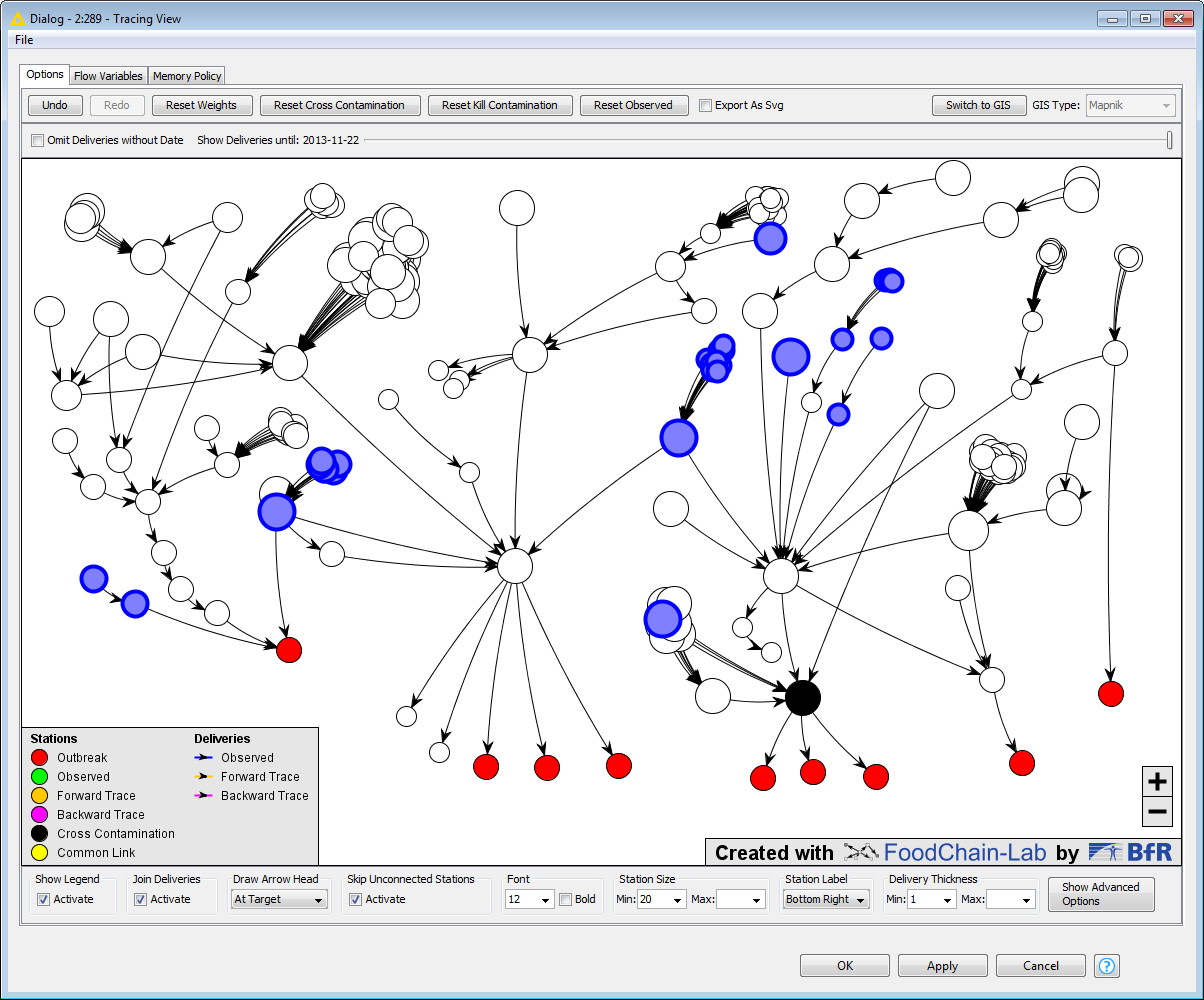
\includegraphics[height=0.6\textheight]{6.png}
	\end{center}
	\begin{itemize}
		\item The blue stations are the ones you selected in the geographical view, since changes you make in one view are automatically applied to the other view.
		\item That makes it easy to switch back and forth between both representations, enabling you to use the benefits of both.
	\end{itemize}
\end{frame}

\section{7}
\begin{frame}
	\begin{center}
  		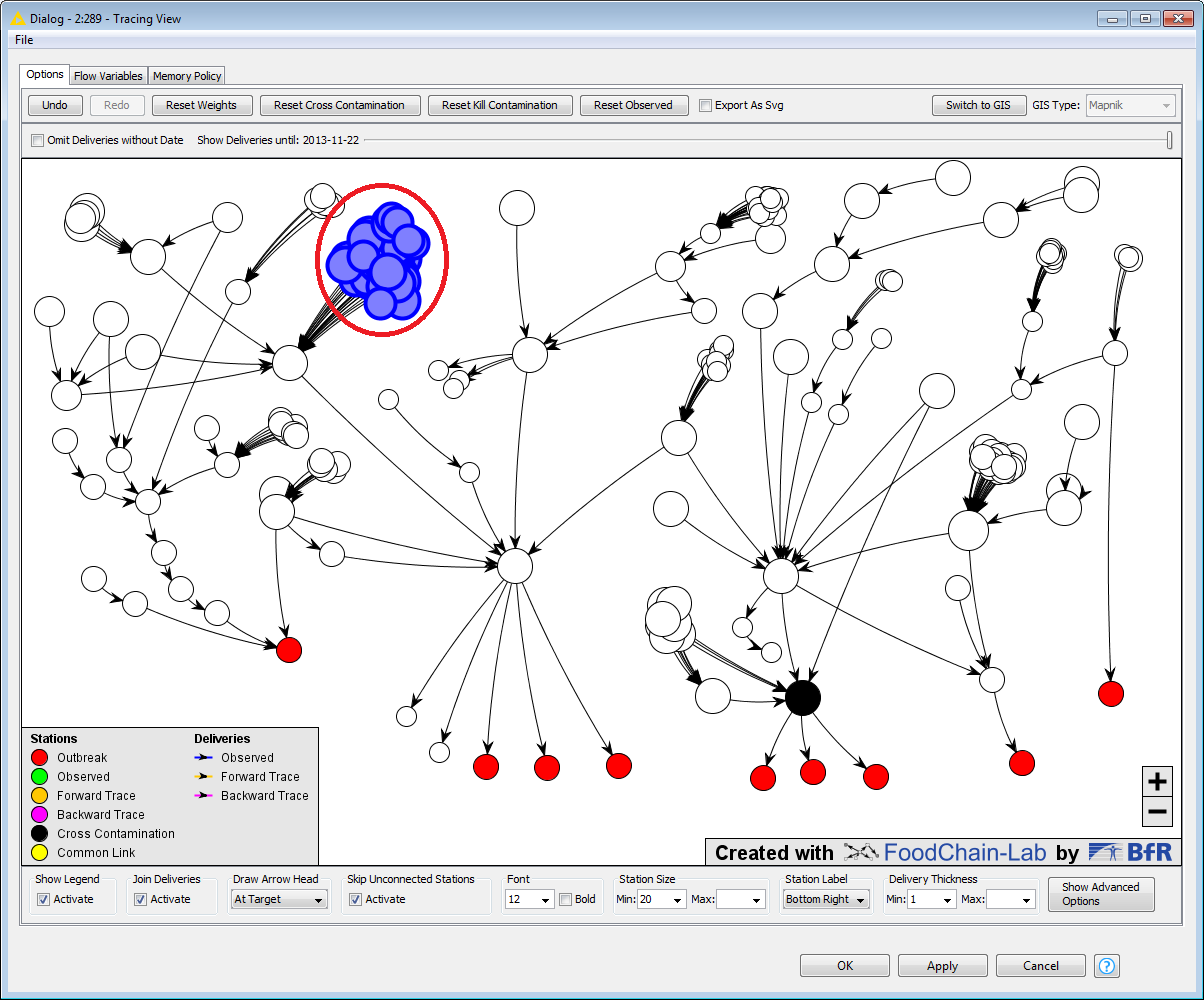
\includegraphics[height=0.6\textheight]{7.png}
	\end{center}
	\begin{itemize}
		\item Lets now select a certain ``cluster'' in the graphical view and see where the stations are in the geographical view.
		\item So select the ``cluster'' in the red circle and click ``Switch to GIS''.
	\end{itemize}
\end{frame}

\section{8}
\begin{frame}
	\begin{center}
  		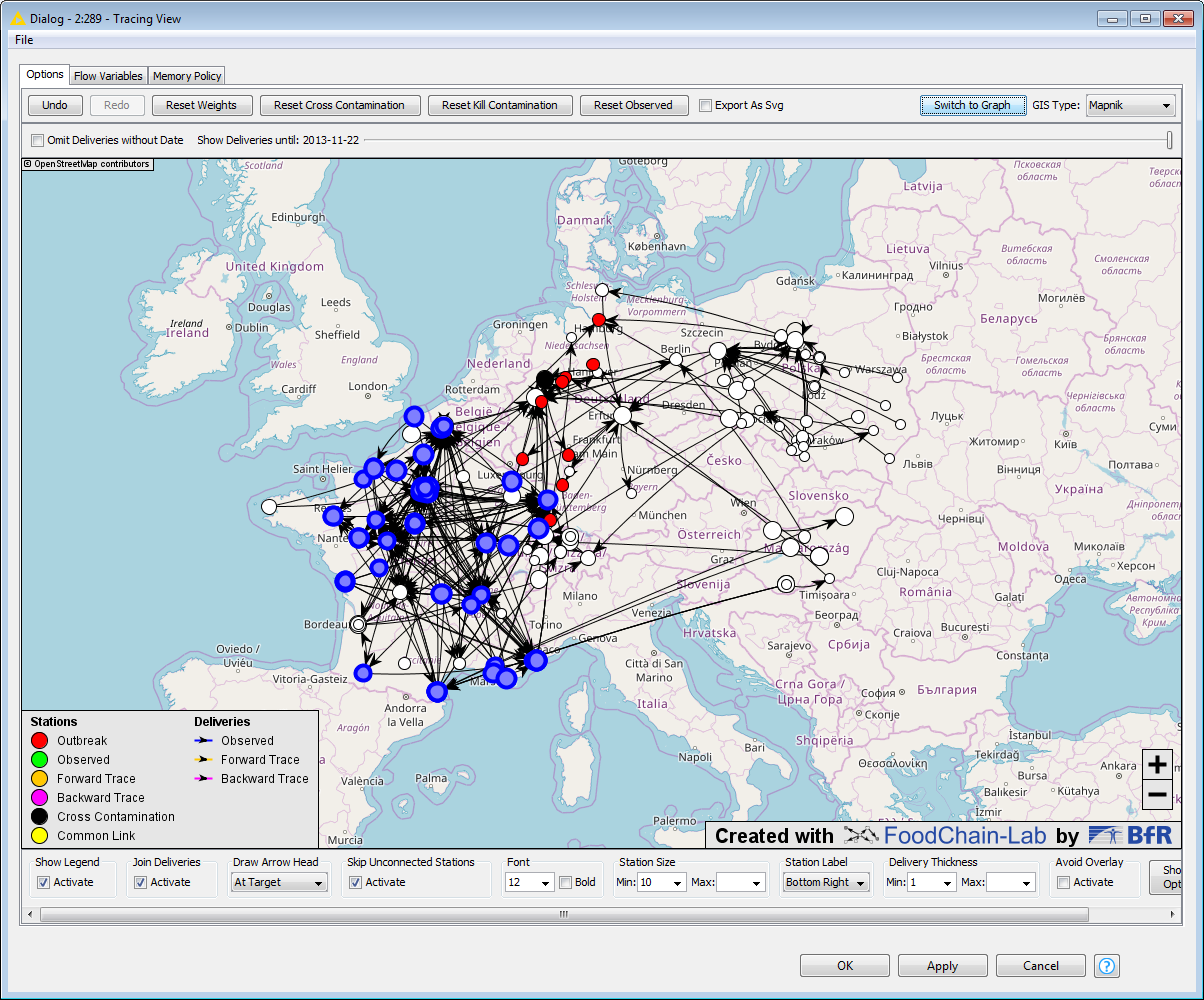
\includegraphics[height=0.6\textheight]{8.png}
	\end{center}
	\begin{itemize}
		\item As you can see the stations of the cluster are located all over France.
	\end{itemize}
\end{frame}

\end{document}
